\chapter{Results and discussion}

Table \eqref{tab:rawdata} shows the raw data from January of 2001 to December of 2012. The initial data collected were from January 2001 to December 2011. The rainfall data for January 2012 to December 2012 were collected after one year for comparison of the predicted values. The data for May 2006 was initially missing. Using bootstrapping method in \texttt{R}, the missing May 2006 data was generated.

\begin{table}[!ht]
\caption{Amount of Precipitation Per Month in mm, from 2001 to 2012}
\begin{threeparttable}
\resizebox{\linewidth}{!}{
\pgfplotstabletypeset[header=true,
font=\small,
every head row/.style={
before row=\toprule,
after row=\midrule,
},
every last row/.style={
after row=\bottomrule},
string type
]{rawdata.dat}
}
\begin{tablenotes}
\item [$\star$] Trace amount, $< 0.01$ mm
\item [$\triangle$] Bootstrapped value
\end{tablenotes}
\end{threeparttable}
\label{tab:rawdata}
\end{table}

\section*{Analysis of Data}

The data was saved in a file named \texttt{baguiorainfall.dat}. This data was then inputted in \Rstat{} and stored in a variable \texttt{baguiorainseries} using the \texttt{ts} function.

\begin{Schunk}
\begin{Sinput}
baguiorain <- read.table("baguiorainfall.dat")
baguiorainseries <- ts(baguiorain, frequency = 12, start = c(2001, 1))
\end{Sinput}
\end{Schunk}


Figure \eqref{fig:TSPlot} shows the graph of the rain fall time series from January 2001 to December 2011. It can be seen that the data is seasonal, peaking every July to August every year.

\begin{figure}[!ht]
\centering
\begin{Schunk}
\begin{Sinput}
plot.ts(baguiorainseries)
\end{Sinput}

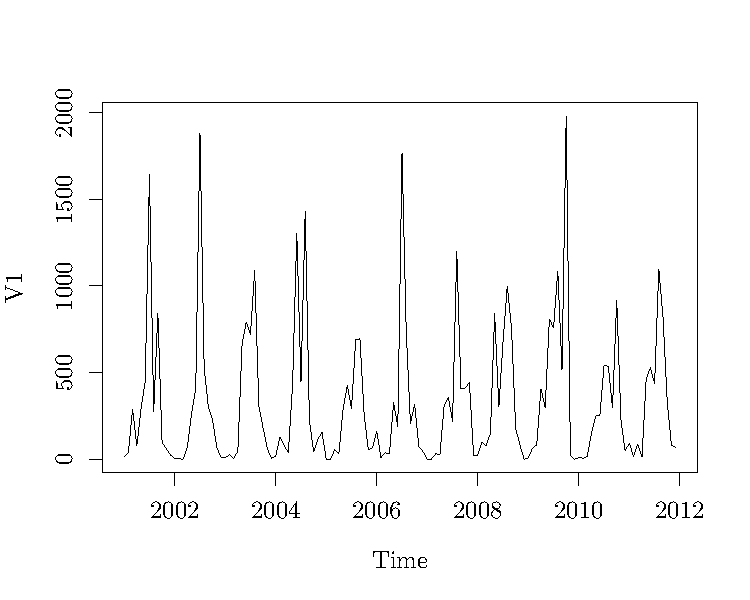
\includegraphics[width=.7\textwidth]{figure/listings-YeastBoxPlot} \end{Schunk}


\caption{\label{fig:TSPlot} Plot of Baguio rain fall time series, from January 2001 to December 2011.}
\end{figure}

Here, the time series data is broken down into its components. This is done in preparation to eliminating the seasonal component of the data. Only the partial results are shown in \eqref{fig:Components}. The full results are in Listing \eqref{fig:Components2}.

\begin{center}
\captionof{figure}{\label{fig:Components} Partial results of the seasonal, trend, and random components.}
\begin{Schunk}
\begin{Sinput}
baguiorainseriescomponents <- decompose(baguiorainseries)
baguiorainseriescomponents
\end{Sinput}
\begin{Soutput}
$x
          Jan      Feb      Mar      Apr      May      Jun      Jul
2001   14.600   39.500  289.800   76.000  291.000  451.400 1642.000
2002    5.000    2.000    0.600   71.200  264.400  411.000 1883.400
2003    9.800   25.400    4.800   46.800  662.700  792.400  721.300
.
.
.

          Aug      Sep      Oct      Nov      Dec
2001  274.000  842.200   97.000   61.600   23.200
2002  525.600  301.500  224.800   67.300   10.000
2003 1089.400  303.200  179.700   60.400    4.400
.
.
.

$seasonal
         Jan     Feb     Mar     Apr     May     Jun     Jul     Aug
2001 -296.55 -293.19 -283.56 -235.99   80.13  204.37  561.21  522.65
2002 -296.55 -293.19 -283.56 -235.99   80.13  204.37  561.21  522.65
2003 -296.55 -293.19 -283.56 -235.99   80.13  204.37  561.21  522.65
.
.
.
         Sep     Oct     Nov     Dec
2001  122.05  128.05 -212.33 -296.84
2002  122.05  128.05 -212.33 -296.84
2003  122.05  128.05 -212.33 -296.84
.
.
.

$trend
       Jan   Feb   Mar   Apr   May   Jun   Jul   Aug   Sep   Oct   Nov
2001    NA    NA    NA    NA    NA    NA 341.5 339.5 325.9 313.6 312.3
2002 317.9 338.4 326.4 309.2 314.8 314.4 314.1 315.3 316.4 315.6 331.2
2003 331.1 306.2 329.8 327.9 325.8 325.3 325.3 329.9 337.4 340.1 330.0
.
.
.

       Dec
2001 309.5
2002 363.7
2003 341.6
.
.
.

$random
          Jan      Feb      Mar      Apr      May      Jun      Jul
2001       NA       NA       NA       NA       NA       NA  739.334
2002  -16.360  -43.257  -42.248   -2.012 -130.491 -107.820 1008.092
2003  -24.773   12.401  -41.398  -45.158  256.792  262.771 -165.233
.
.
.

          Aug      Sep      Oct      Nov      Dec
2001 -588.150  394.268 -344.686  -38.390   10.510
2002 -312.329 -136.973 -218.836  -51.528  -56.807
2003  236.821 -156.201 -288.458  -57.242  -40.400
.
.
.

$figure
 [1] -296.55 -293.19 -283.56 -235.99   80.13  204.37  561.21  522.65
 [9]  122.05  128.05 -212.33 -296.84

$type
[1] "additive"

attr(,"class")
[1] "decomposed.ts"
\end{Soutput}
\end{Schunk}
\end{center}

It can be seen in Figure \eqref{fig:Components} that the data is of additive type. The plot is in Figure \eqref{fig:ComponentsPlot}. 

\begin{figure}[!ht]
\centering
\begin{Schunk}
\begin{Sinput}
plot(baguiorainseriescomponents)
\end{Sinput}

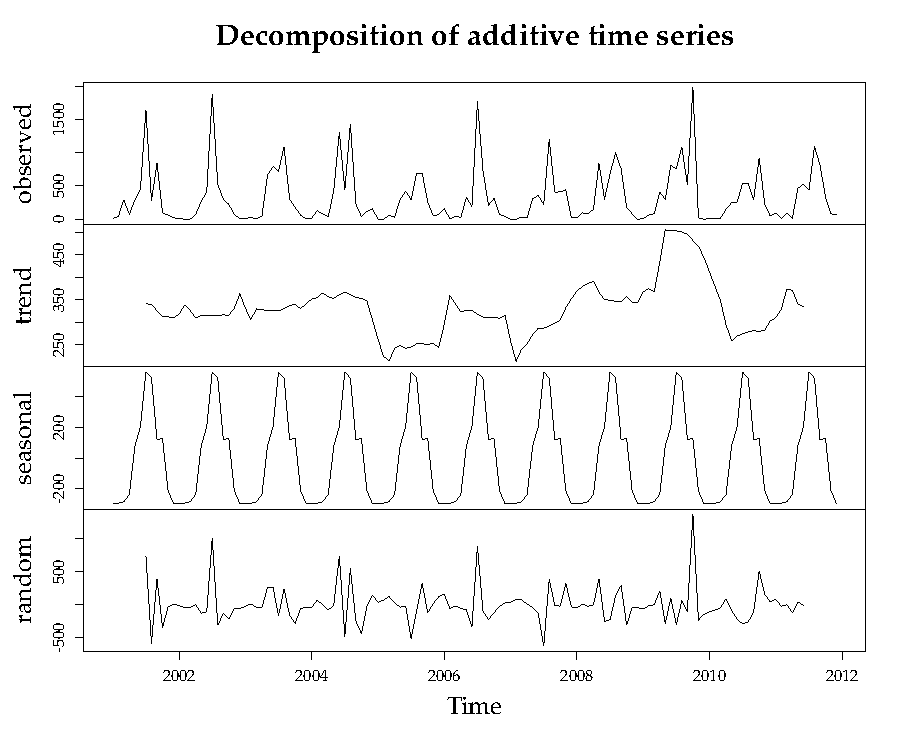
\includegraphics[width=.7\textwidth]{figure/listings-ComponentsPlot} \end{Schunk}


\caption{\label{fig:ComponentsPlot} The plot of the components of the rainfall time series data.}
\end{figure}

To use exponential smoothing to make forecasts for the time series of monthly rainfall in Baguio City, the \texttt{HoltWinters()} function was used.

\begin{figure}[!ht]
\begin{Sinput}
rainforecasts <- HoltWinters(raintimeseries)
rainforecasts
\end{Sinput}
\begin{Soutput}
Holt-Winters exponential smoothing with trend and additive seasonal component.

Call:
 HoltWinters(x = raintimeseries) 

Smoothing parameters:
 alpha:  0.001826 
 beta :  0.422 
 gamma:  0.3554 

Coefficients:
         [,1]
a    267.1477
b      0.5062
s1  -208.3311
s2  -227.2503
s3  -194.1851
s4  -136.7234
s5   147.8871
s6   216.3476
s7   338.7154
s8   673.8567
s9   321.0458
s10  430.4775
s11 -130.6776
s12 -215.8636
\end{Soutput}
\caption{\label{fig:HoltWSmoothing} The output of \texttt{HoltWinters()} function.}
\end{figure}

The output of \texttt{HoltWinters()} made forecast for the same time period covered by the original time series, the time series included rainfall for Baguio City for the period January 2000 to December 2011. So the forecasts were also for that period. An $\alpha$ of 0.001826 indicates that the forecasts were based on both recent and less recent observations--although somewhat more weight was placed on recent observations (Coghlan 2011). A $\beta$ of $0.422$ and a low $\gamma$ of 0.3554 meant that the estimate
of both the trend and seasonal components at the current time point are based upon both recent
observations and some observations in the more distant past. The graph of the original time series against the fitted forecast of the model can be seen in Figure \eqref{fig:fittedgraph}.
\newpage
\begin{center}
\begin{Schunk}
\begin{Sinput}
plot(baguiorainseriesforecasts)
\end{Sinput}

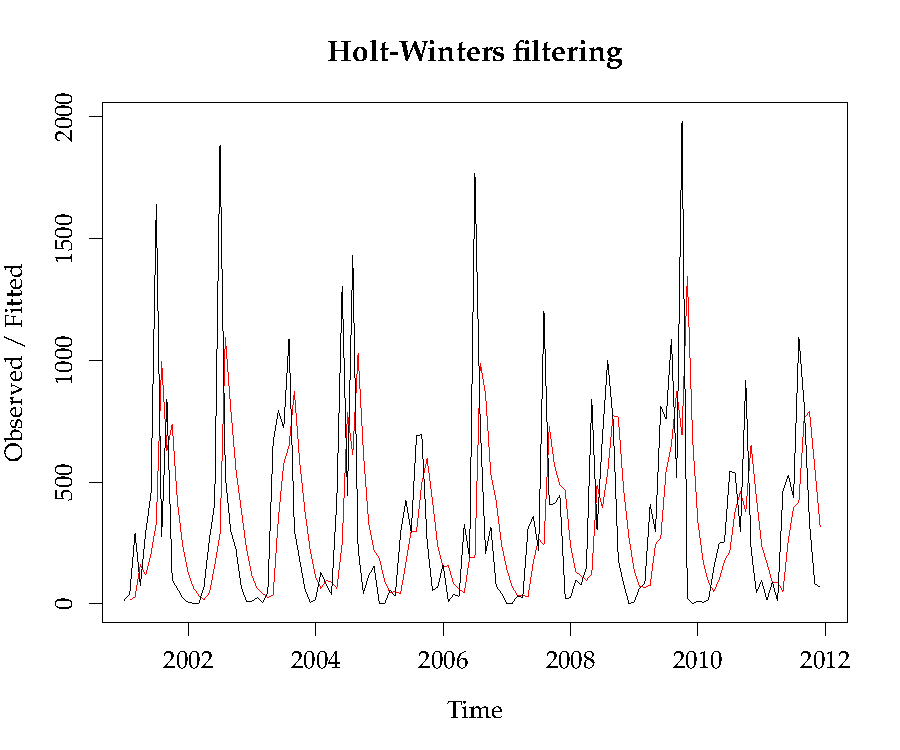
\includegraphics[width=.7\textwidth]{figure/listings-fittedgraph} \end{Schunk}

\captionof{figure}{\label{fig:fittedgraph} The original rainfall time series with the predicted values of the derived model in the same period.}
\end{center}

The output of \texttt{HoltWinters()} function was stored in the variable\newline \texttt{baguiorainseriesforecasts\$fitted}. The forecast for the period January 2000 to December 2011 is shown partially in Figure \eqref{fig:fitted}, and in full in Figure \eqref{fig:fitted2} of \textbf{Appendix B}.

\begin{figure}[!ht]
\begin{Schunk}
\begin{Sinput}
baguiorainseriesforecasts$fitted
\end{Sinput}
\begin{Soutput}
            xhat   level
Feb 2001   14.60   14.60
Mar 2001   27.22   27.22
Apr 2001  160.31  160.31
May 2001  117.58  117.58
Jun 2001  205.48  205.48
.
.
.
Oct 2011  790.45  790.45
Nov 2011  558.28  558.28
Dec 2011  316.67  316.67
\end{Soutput}
\end{Schunk}

\caption{\label{fig:fitted} The forecast for the period January 2000 to December 2011 using Holt Winters.}
\end{figure}

We now make forecasts for further time points by using the
\texttt{forecast.HoltWinters()} function in the R \texttt{forecast} package. \texttt{forecast.HoltWinters()} uses the predictive model derived using the HoltWinters() function. The result is in Figure \eqref{fig:Forecast2}.

\begin{center}
\begin{Schunk}
\begin{Sinput}
library(forecast)
\end{Sinput}
\begin{Soutput}
This is forecast 4.01 
\end{Soutput}
\begin{Sinput}
baguiorainseriesforecasts2 <- forecast.HoltWinters(baguiorainseriesforecasts, 
    h = 12)
baguiorainseriesforecasts2
\end{Sinput}
\begin{Soutput}
         Point Forecast   Lo 80  Hi 80   Lo 95  Hi 95
Jan 2012          59.32 -366.29  484.9 -591.60  710.2
Feb 2012          40.91 -384.70  466.5 -610.01  691.8
Mar 2012          74.48 -351.14  500.1 -576.44  725.4
Apr 2012         132.45 -293.17  558.1 -518.48  783.4
May 2012         417.57   -8.06  843.2 -233.37 1068.5
Jun 2012         486.53   60.90  912.2 -164.42 1137.5
Jul 2012         609.41  183.77 1035.0  -41.56 1260.4
Aug 2012         945.05  519.40 1370.7  294.07 1596.0
Sep 2012         592.75  167.08 1018.4  -58.25 1243.7
Oct 2012         702.69  277.01 1128.4   51.66 1353.7
Nov 2012         142.04 -283.66  567.7 -509.02  793.1
Dec 2012          57.36 -368.37  483.1 -593.73  708.4
\end{Soutput}
\end{Schunk}
\begin{Sinput}
rainforecasts$SSE
\end{Sinput}
\begin{Soutput}
[1] 13193425
\end{Soutput}


\captionof{figure}{\label{fig:Forecast2} The 12-month forecast for the year 2012 based on \texttt{Holt Winters} smoothing.}
\end{center}

Figure \eqref{fig:predgraph} shows the original time series with the graph of the predicted values (in blue color) and the low and high values (shown in light blue-gray color).

\begin{center}
\centering
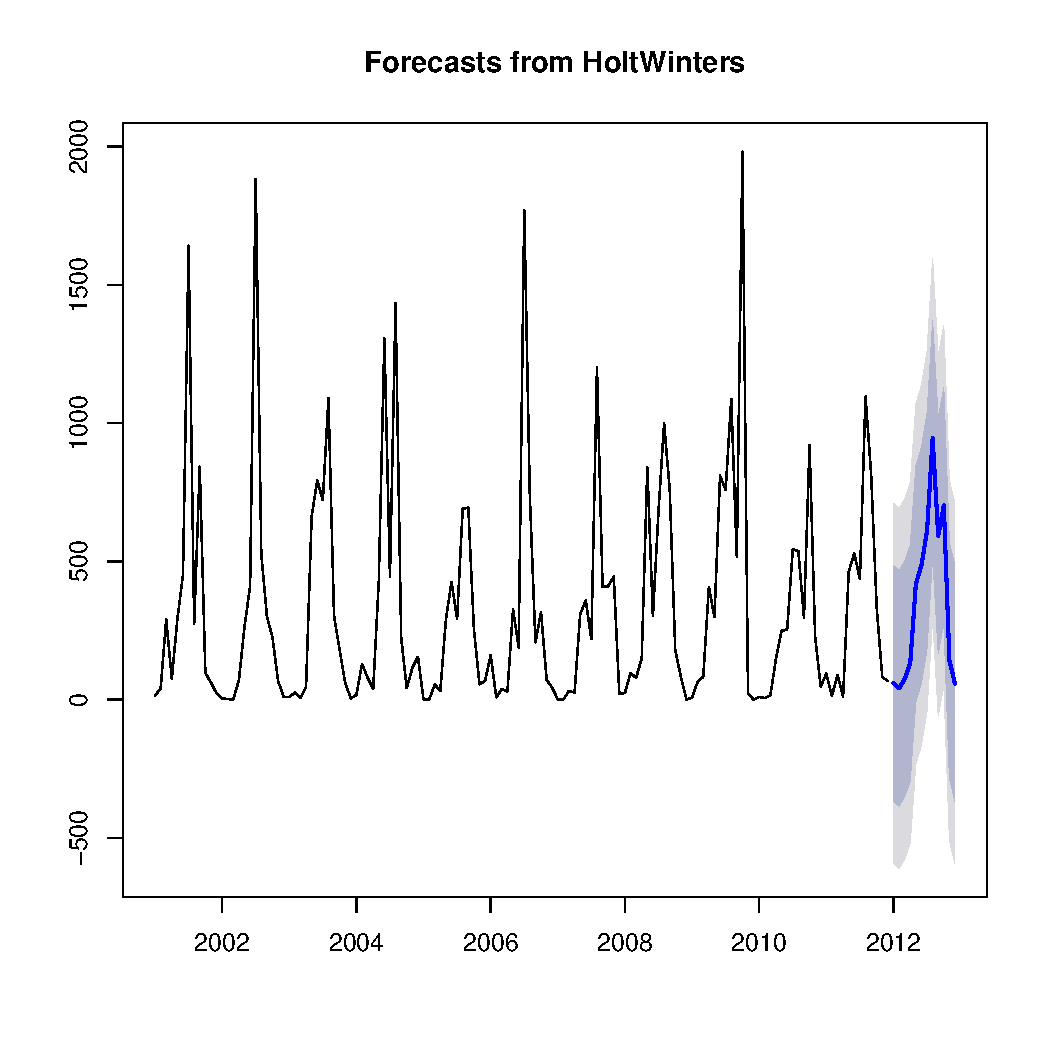
\includegraphics[width=0.7\maxwidth,height=3.5in]{figure/listings-HWComputations3}
\captionof{figure}{\label{fig:predgraph} The graph of the time series with the forecasted values.}
\end{center}

The ‘forecast errors’ are calculated as the observed values minus predicted values, for each time point. We can
only calculate the forecast errors for the time period covered by our original time series, which is January 2011 to December 2011 for
the rainfall data. One measure of the accuracy of the predictive model is the sum-of-squared-
errors (SSE) for the in-sample forecast errors.
The in-sample forecast errors are stored in the named element “residuals” of the list variable returned by \texttt{forecast.HoltWinters()}. If the predictive model cannot be improved upon, there should be no correlations between
forecast errors for successive predictions. In other words, if there are correlations between forecast errors for
successive predictions, it is likely that the  exponential smoothing forecasts could be improved upon by
another forecasting technique. The function \texttt{acf()} function was used here to test for autocorrelation in the errors.

\begin{Sinput}
acf(rainforecasts2$residuals, lag.max = 20)
\end{Sinput}

\begin{center}
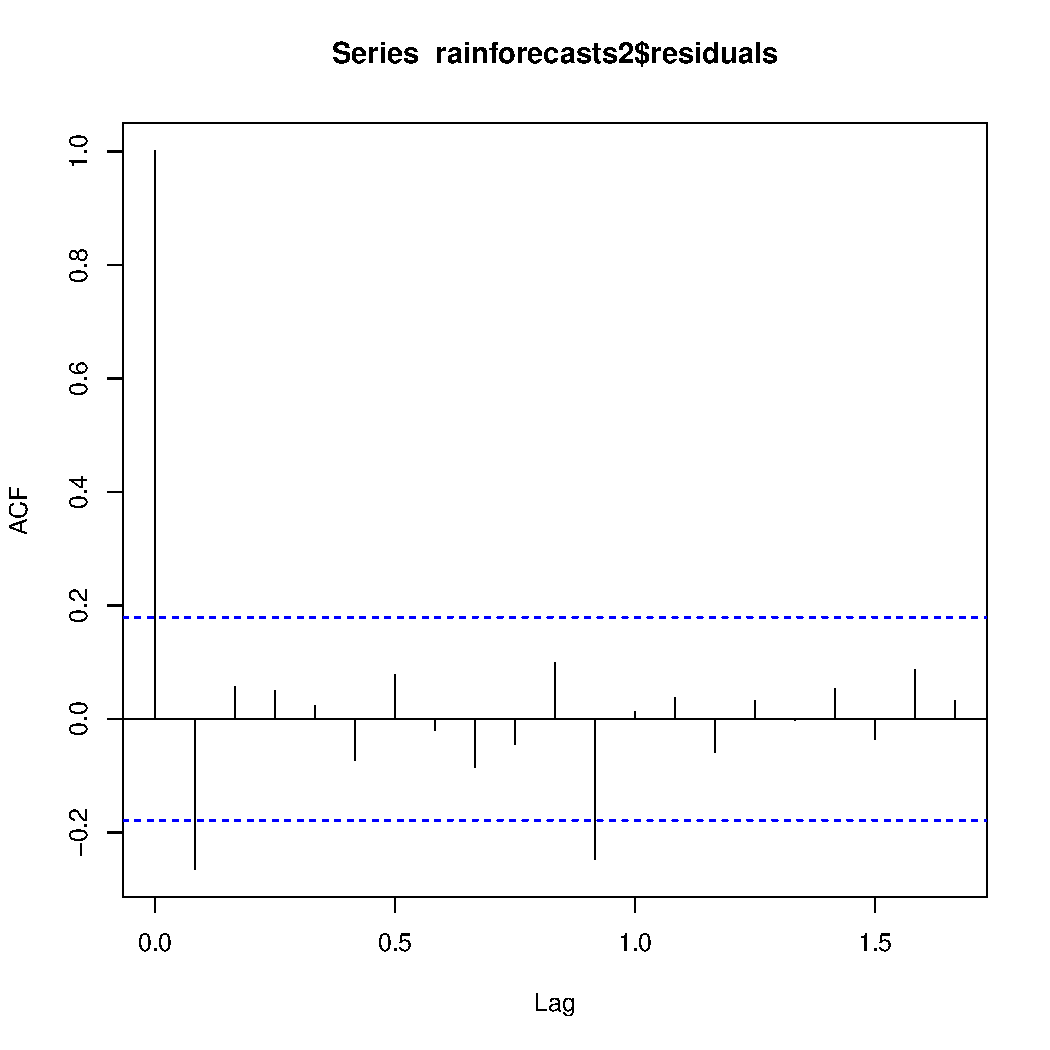
\includegraphics[width=0.7\maxwidth,height=3.5in]{figure/listings-HWComputations4}
\captionof{figure}{\label{fig:acf} \texttt{acf()} output.}
\end{center}

Here the correlogram shows that the sample autocorrelation for the in-sample forecast errors at lags 1 and 11 exceed
the significance bounds. This is more than the 1 than the one in 20 of the autocorrelations for the first twenty lags to
exceed the 95\% significance bounds by chance alone indicating possible auto-correlation in internal errors. 

\begin{Sinput}
Box.test(rainforecasts2$residuals, lag = 20, type = "Ljung-Box")
\end{Sinput}
\begin{Soutput}

	Box-Ljung test

data:  rainforecasts2$residuals 
X-squared = 23.91, df = 20, p-value = 0.2465
\end{Soutput}
\begin{Sinput}
plot.ts(rainforecasts2$residuals)
\end{Sinput}

The Ljung-Box test, with p-value of 0.2465 on the other hand shows no evidence of non-zero autocorrelations in the in-sample forecast errors at lags 1-20.

To be sure that the predictive model cannot be improved upon, the researchers checked whether the forecast errors are normally distributed with mean zero and constant variance. To check whether the forecast errors have
constant variance, the researchers made a time plot of the in-sample forecast errors:

\begin{center}
\begin{Sinput}
plot.ts(rainforecasts2$residuals)
\end{Sinput}

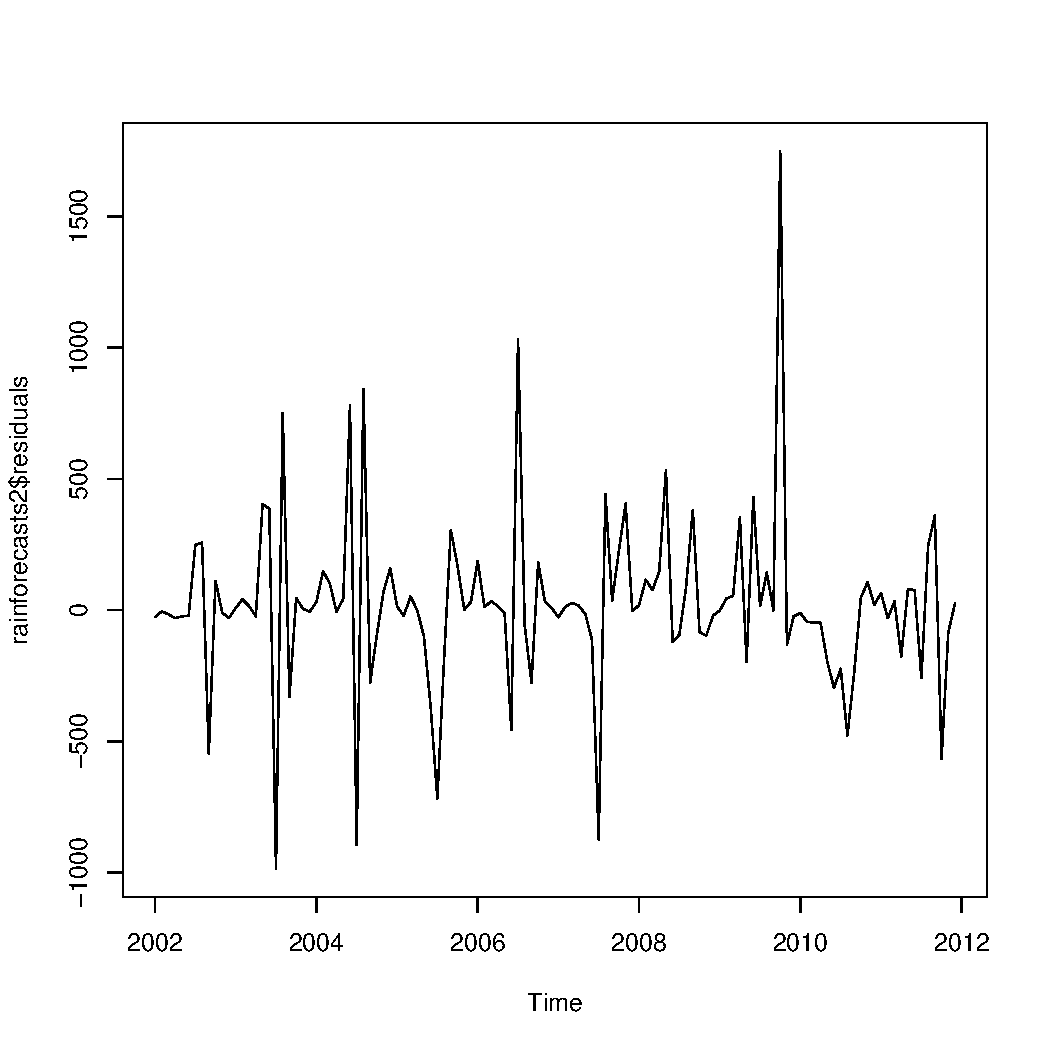
\includegraphics[width=0.7\maxwidth, height=3.5in]{figure/listings-HWComputations5}
\captionof{figure}{\label{insampleerrors}Plot of the in-sample forecast errors.}
\end{center}

The plot shows that the in-sample forecast errors seem to have roughly constant variance over time with some fluctuations between 2000 and 2011.

To check whether the forecast errors are normally distributed with mean zero, a histogram of the forecast errors, with an overlaid normal curve that has mean zero and the same standard deviation as the distribution
of forecast errors can be plotted. Here the R function \texttt{plotForecastErrors()} was used.

\begin{Sinput}
plotForecastErrors <- function(forecasterrors) {
    # make a red histogram of the forecast errors:
    mybinsize <- IQR(forecasterrors)/4
    mymin <- min(forecasterrors) * 3
    mymax <- max(forecasterrors) * 3
    mybins <- seq(mymin, mymax, mybinsize)
    hist(forecasterrors, col = "red", freq = FALSE, breaks = mybins)
    # freq=FALSE ensures the area under the histogram = 1
    mysd <- sd(forecasterrors)
    # generate normally distributed data with mean 0 and standard deviation
    # mysd
    mynorm <- rnorm(10000, mean = 0, sd = mysd)
    myhist <- hist(mynorm, plot = FALSE, breaks = mybins)
    # plot the normal curve as a blue line on top of the histogram of
    # forecast errors:
    points(myhist$mids, myhist$density, type = "l", col = "blue", lwd = 2)
}
plotForecastErrors(rainforecasts2$residuals)
\end{Sinput}

\begin{center}
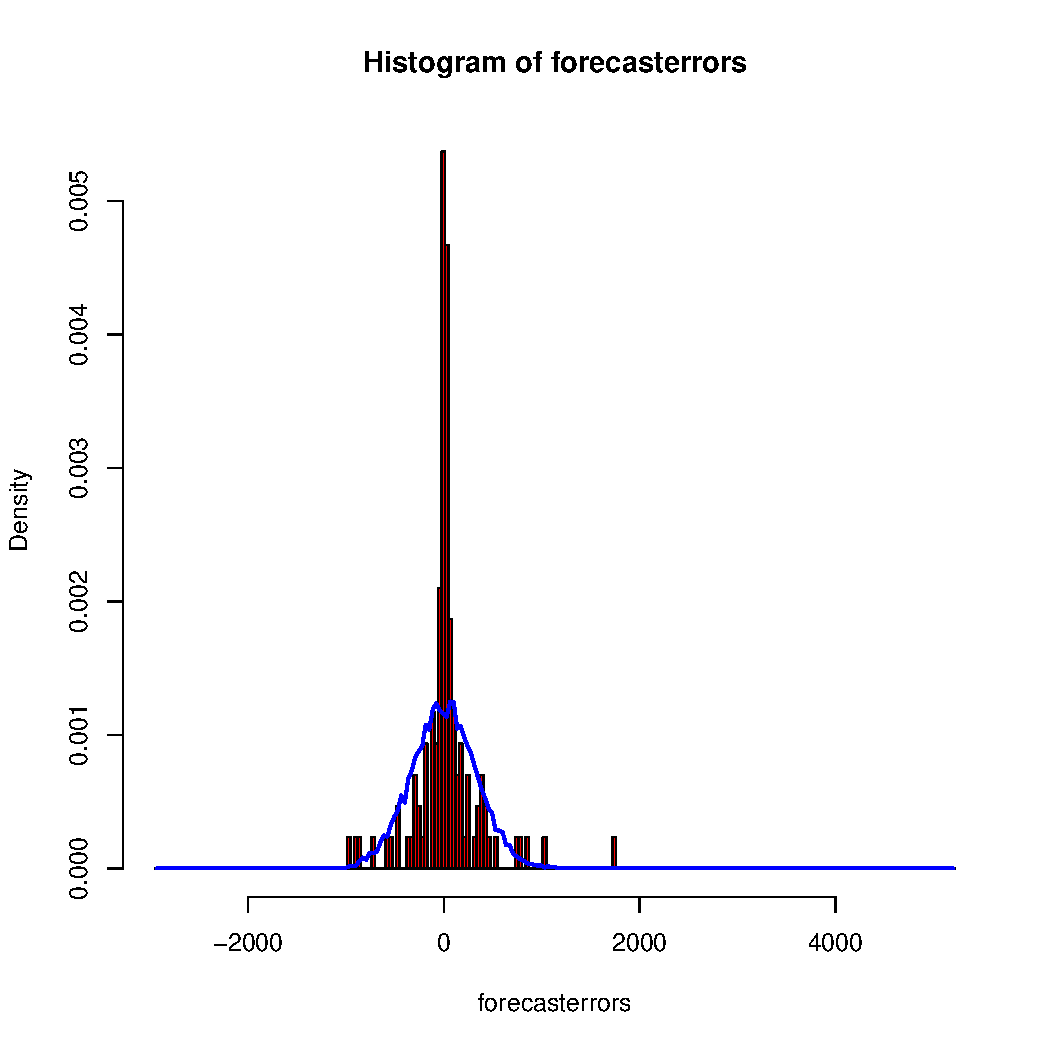
\includegraphics[width=0.7\maxwidth,height=3.5in]{figure/listings-HWComputations6}
\captionof{figure}{\label{fig:normalplot} A histogram of the forecast errors, with an overlaid normal curve that has mean zero and the same standard deviation as the distribution of forecast errors.}
\end{center}

The plot shows that the distribution of forecast errors is roughly centred on zero, and is more or less normally
distributed, although it seems to be slightly skewed to the right compared to a normal curve. However, the right
skew is relatively small, and so it is plausible that the forecast errors are normally distributed with mean zero.

%Finally, we use t-test for the predicted values and the actual values for 2012 taken from PAGASA.
%
%\begin{Sinput}
%actual <- c(17.5, 80.3, 151.9, 72.6, 207.7, 659, 1020.2, 2207, 288.3, 72.4, 
%    57.8, 10.8)
%predicted <- c(59.32, 40.91, 74.48, 132.45, 417.57, 486.53, 609.41, 945.05, 
%    592.75, 702.69, 142.69, 57.36)
%compared <- data.frame(actual, predicted)
%attach(compared)
%\end{Sinput}
%\begin{Soutput}
%The following object(s) are masked _by_ '.GlobalEnv':
%
%    actual, predicted
%\end{Soutput}
%\begin{Sinput}
%t.test(actual, predicted, data = compared, var.equal = TRUE)
%\end{Sinput}
%\begin{Soutput}
%
%	Two Sample t-test
%
%data:  actual and predicted 
%t = 0.236, df = 22, p-value = 0.8156
%alternative hypothesis: true difference in means is not equal to 0 
%95 percent confidence interval:
% -379.2  476.6 
%sample estimates:
%mean of x mean of y 
%    403.8     355.1 
%\end{Soutput}
%
%The t test shows that the predicted values and the 2012 rainfall data have no significant difference at the significance level $\alpha=0.05$. 